\documentclass{beamer}
\usepackage{amsmath,amssymb,amsfonts}
\usepackage{graphicx}
\graphicspath{ {../} }

% \usepackage{beamerthemesplit} // Activate for custom appearance

\title{Spectral Graph Layout}
\author{Wilmer Uruchi}
\date{\today}

\begin{document}

\frame{\titlepage}

\section[Outline]{}
\frame{\tableofcontents}

\section{Spectral Graph Layout} 
\subsection{Theoretical details}
\frame{
	\frametitle{Brief Description}
Spectral Graph Layout is a technique that attempts to produce nice looking graph drawings in a reasonable time using algebraic properties of the Laplacian Matrix of the Graph. 

For this implementation we are using the Degree Normalized Graph Laplacian and in further experimentation, we are adding some weights into the equation.


}
\frame{
	\frametitle{2 Main Advantages}
	\begin{itemize}
	\item It provides an exact solution with a mathematically-sound formulation.
	\item It is fast.
	\end{itemize}
}
\subsection{Some Background}
\frame{
 	\frametitle{The Adjacency Matrix}
	
	The adjacency matrix of the graph $G(V,E)$ is the symmetric $n \times n$ matrix $A$, where:
	
	\begin{equation}
  	A_{ij} =
    	\begin{cases}
      		0 & \text{$(i,i) \notin E$}\\
      		w_{ij} & \text{$(i,j) \in E$} \\
    	\end{cases}       
	\end{equation}
}
\frame{
	\frametitle{The Degrees Matrix}
	
	The degrees matrix of the graph $G(V,E)$ is the $n \times n$ diagonal matrix $A$, where:
	
	\begin{equation}
  	D_{ii} = deg(i)       
	\end{equation}
}

\frame{
	\frametitle{The Graph Laplacian Matrix}
	$$L = D - A$$
	
	The Laplacian is a symmetric $n \times n$ matrix associated with the graph $L$, where:
	
	\begin{equation}
  	L_{ij} =
    	\begin{cases}
      		deg(i) & \text{$i = i$}\\
      		0 & \text{$i \neq j$} \\
		-w_{ij} & \text{$(i,j) \in E$} \\
    	\end{cases}       
	\end{equation}
}

\frame{
	\frametitle{Some useful features of The Laplacian}
	\begin{itemize}
	\item $L$ is real symmetric, hence, its $n$ eigenvalues are real and its eigenvectors are orthogonal.
	\item $L$ is positive semidefinite, so all eigenvalues of $L$ are nonnegative.
	\item $1_{n} = (1,1, \dots, 1)^{T} \in \mathbb{R}^{n}$ is an eigenvector of $L$ associated with the eigenvalue $0$.
	\item The multiplicity of the zero eigenvalue is equal to the number of connected components of $G$. If $G$ is connected, then $1_{n}$ is the only eigenvector associated with eigenvalue $0$.
	\end{itemize}
}

\frame{
	\frametitle{THEOREM 1}
	
	Given a symmetric matrix $A_{n \times n}$, denote by $v^1, \dots, v^n$ its eigenvectors, with corresponding eigenvalues $\lambda_{1} \leq \dots \leq \lambda_{n}$. Then, $v^1, \dots, v^p$ are an optimal solution to the constrained minimization problem:
	
	$$min_{x^1, \dots, x^p} \quad \Sigma_{k=1}^{p} (x^k)^{T} Ax^k$$
	
	Subject to:
	
	$$(x^k)^T x^l = \delta_{kl}$$
	$$k,l = 1, \dots, p$$
	
	In this equation, $\delta_{ij}$ is the Kronecker delta defined as 1 for $i = j$ and $0$ otherwise.
}

\frame{
	\frametitle{THEOREM 2}
	
	Given a symmetric matrix $A_{n \times n}$, and a positive definite matrix $B$, denote by $v^1, \dots, v^n$ the generalized eigenvectors of $(A,B)$, with corresponding eigenvalues $\lambda_{1} \leq \dots \leq \lambda_{n}$. Then, $v^1, \dots, v^p$ are an optimal solution of the constrained minimization problem:
	
	$$min_{x^1, \dots, x^p} \quad \Sigma_{k=1}^{p} (x^k)^{T} Ax^k$$
	
	Subject to:
	
	$$(x^k)^T Bx^l = \delta_{kl}$$
	$$k,l = 1, \dots, p$$
	
}

\subsection{Drawing Using Degree-Normalized Eigenvectors}
\frame
{
  	\frametitle{Some remarks}
	For regular graphs of uniform degree $deg$, the eigenvectors of the Laplacian equal those of the adjacency matrix, but in reversed order, because $L = deg * I - A$, and adding the identity matrix does not change eigenvectors.
	
	For non-regular graphs, use of the Laplacian is based on a more solid theoretical basis, and in practice, gives nicer results than those obtained by the adjacency matrix. 
	
	\textbf{We will focus on visualization using eigenvectors of the Laplacian.}
}
\frame
{
	\frametitle{Motivation}
	\textbf{Autosubmit} is a library that manages experiments sent to HPC platforms, these experiments can contain hundreds of jobs that follow dependency relationships. 
	
	It is important to visualize these dependencies in a \textbf{fast} and understandable way. Also, it would be great if the visualization gives some intuition about the structure of the experiment.
	
	Let's use the degree of each node (job) and the weight of the edges (relationships between jobs) to generate a proper layout.
	
	For more information on the mathematical basis of this approach, review \cite{koren}.
	
}
\frame
{
	\frametitle{Minimization problem +}
	
	For more information on how to get to this form of the minimization problem, review \cite{koren}.
	
	Weighting sums according to node masses:
	\begin{equation}
	min_{x^1, \dots, x^p} \quad \frac{\Sigma_{k=1}^{p} (x^k)^{T} Lx^k}{\Sigma_{k=1}^{p} (x^k)^{T} Dx^k}
	\end{equation}
	
	Subject to:
	
	$$(x^k)^T Dx^l = \delta_{ij} \quad k,l = 1, \dots, p$$
	$$(x^k)^T D1^n = 0  \quad k = 1, \dots, p$$
	
	The optimal solution $u^2, \dots, u^{p+1}$, the generalized eigenvectors of $(L,D)$.
}
\frame
{
	\frametitle{Intuition}
	
	In $(4)$ the denominator moderates the behavior of the numerator. The numerator strives to place the nodes with \textbf{high degree at the center of the drawing}, so that they are in proximity to other nodes. On the other hand, the denominator also emphasizes those nodes with high degrees, but in a reversed way; it strives to \textbf{enlarge their scatter}. Thus, we get a drawing more balanced, preventing a situation in which nodes with lower degree are excessively separated from the rest of the nodes.
	
}

\subsection{The algorithm}
\frame{
	\frametitle{Implementation}
	
	Basically:
	\begin{enumerate}
	\item Read information, e.g. from an edge list text file: $u \quad v \quad w_{uv}$
	\item Build Graph $G(V,E)$. 
	\item Build Degree Matrix $D$
	\item Build Adjacency Matrix $A$
	\item Build Degree Normalized Laplacian Matrix $L$
	\item Calculate smallest (Smallest in magnitude eigenvalues) eigenvectors of $L$: $v^2, \dots, v^p$ where $p$ is the number of dimensions.
	\item Set $v^2$ as  x-coordinates, and $v^3$ as y-coordinates.
	\item Draw
	\end{enumerate}
}

\frame{
	\frametitle{Versions}
	
Version $1$ is the drawing with uniform weight across all edges, and version $2$ is the one that considers weights for edges.
	
	Edge $v_i \quad v_j$ has $w_{ij} > 1$ if it is required by the experiment structure that these are grouped more closely together (set as 3 for experimentation).
}

\subsection{Results}
\frame{
	\begin{figure}[h]
	\caption{Experiment a1yw $|V| = 2358 \quad |E| = 7117$. Weighted drawing.}
	\centering
	
\includegraphics[width=0.75\textwidth]{mygraph_a1yw.png}
	\end{figure}
}

\frame{
	\begin{figure}[h]
	\caption{Experiment a1yw $|V| = 2358 \quad |E| = 7117$. Uniform weight drawing.}
	\centering
	
\includegraphics[width=0.75\textwidth]{mygraph_a1yw_nw.png}
	\end{figure}
}

\frame{
	\begin{figure}[h]
	\caption{Experiment a28o $|V| = 1365 \quad |E| = 3775$. Weighted drawing.}
	\centering
	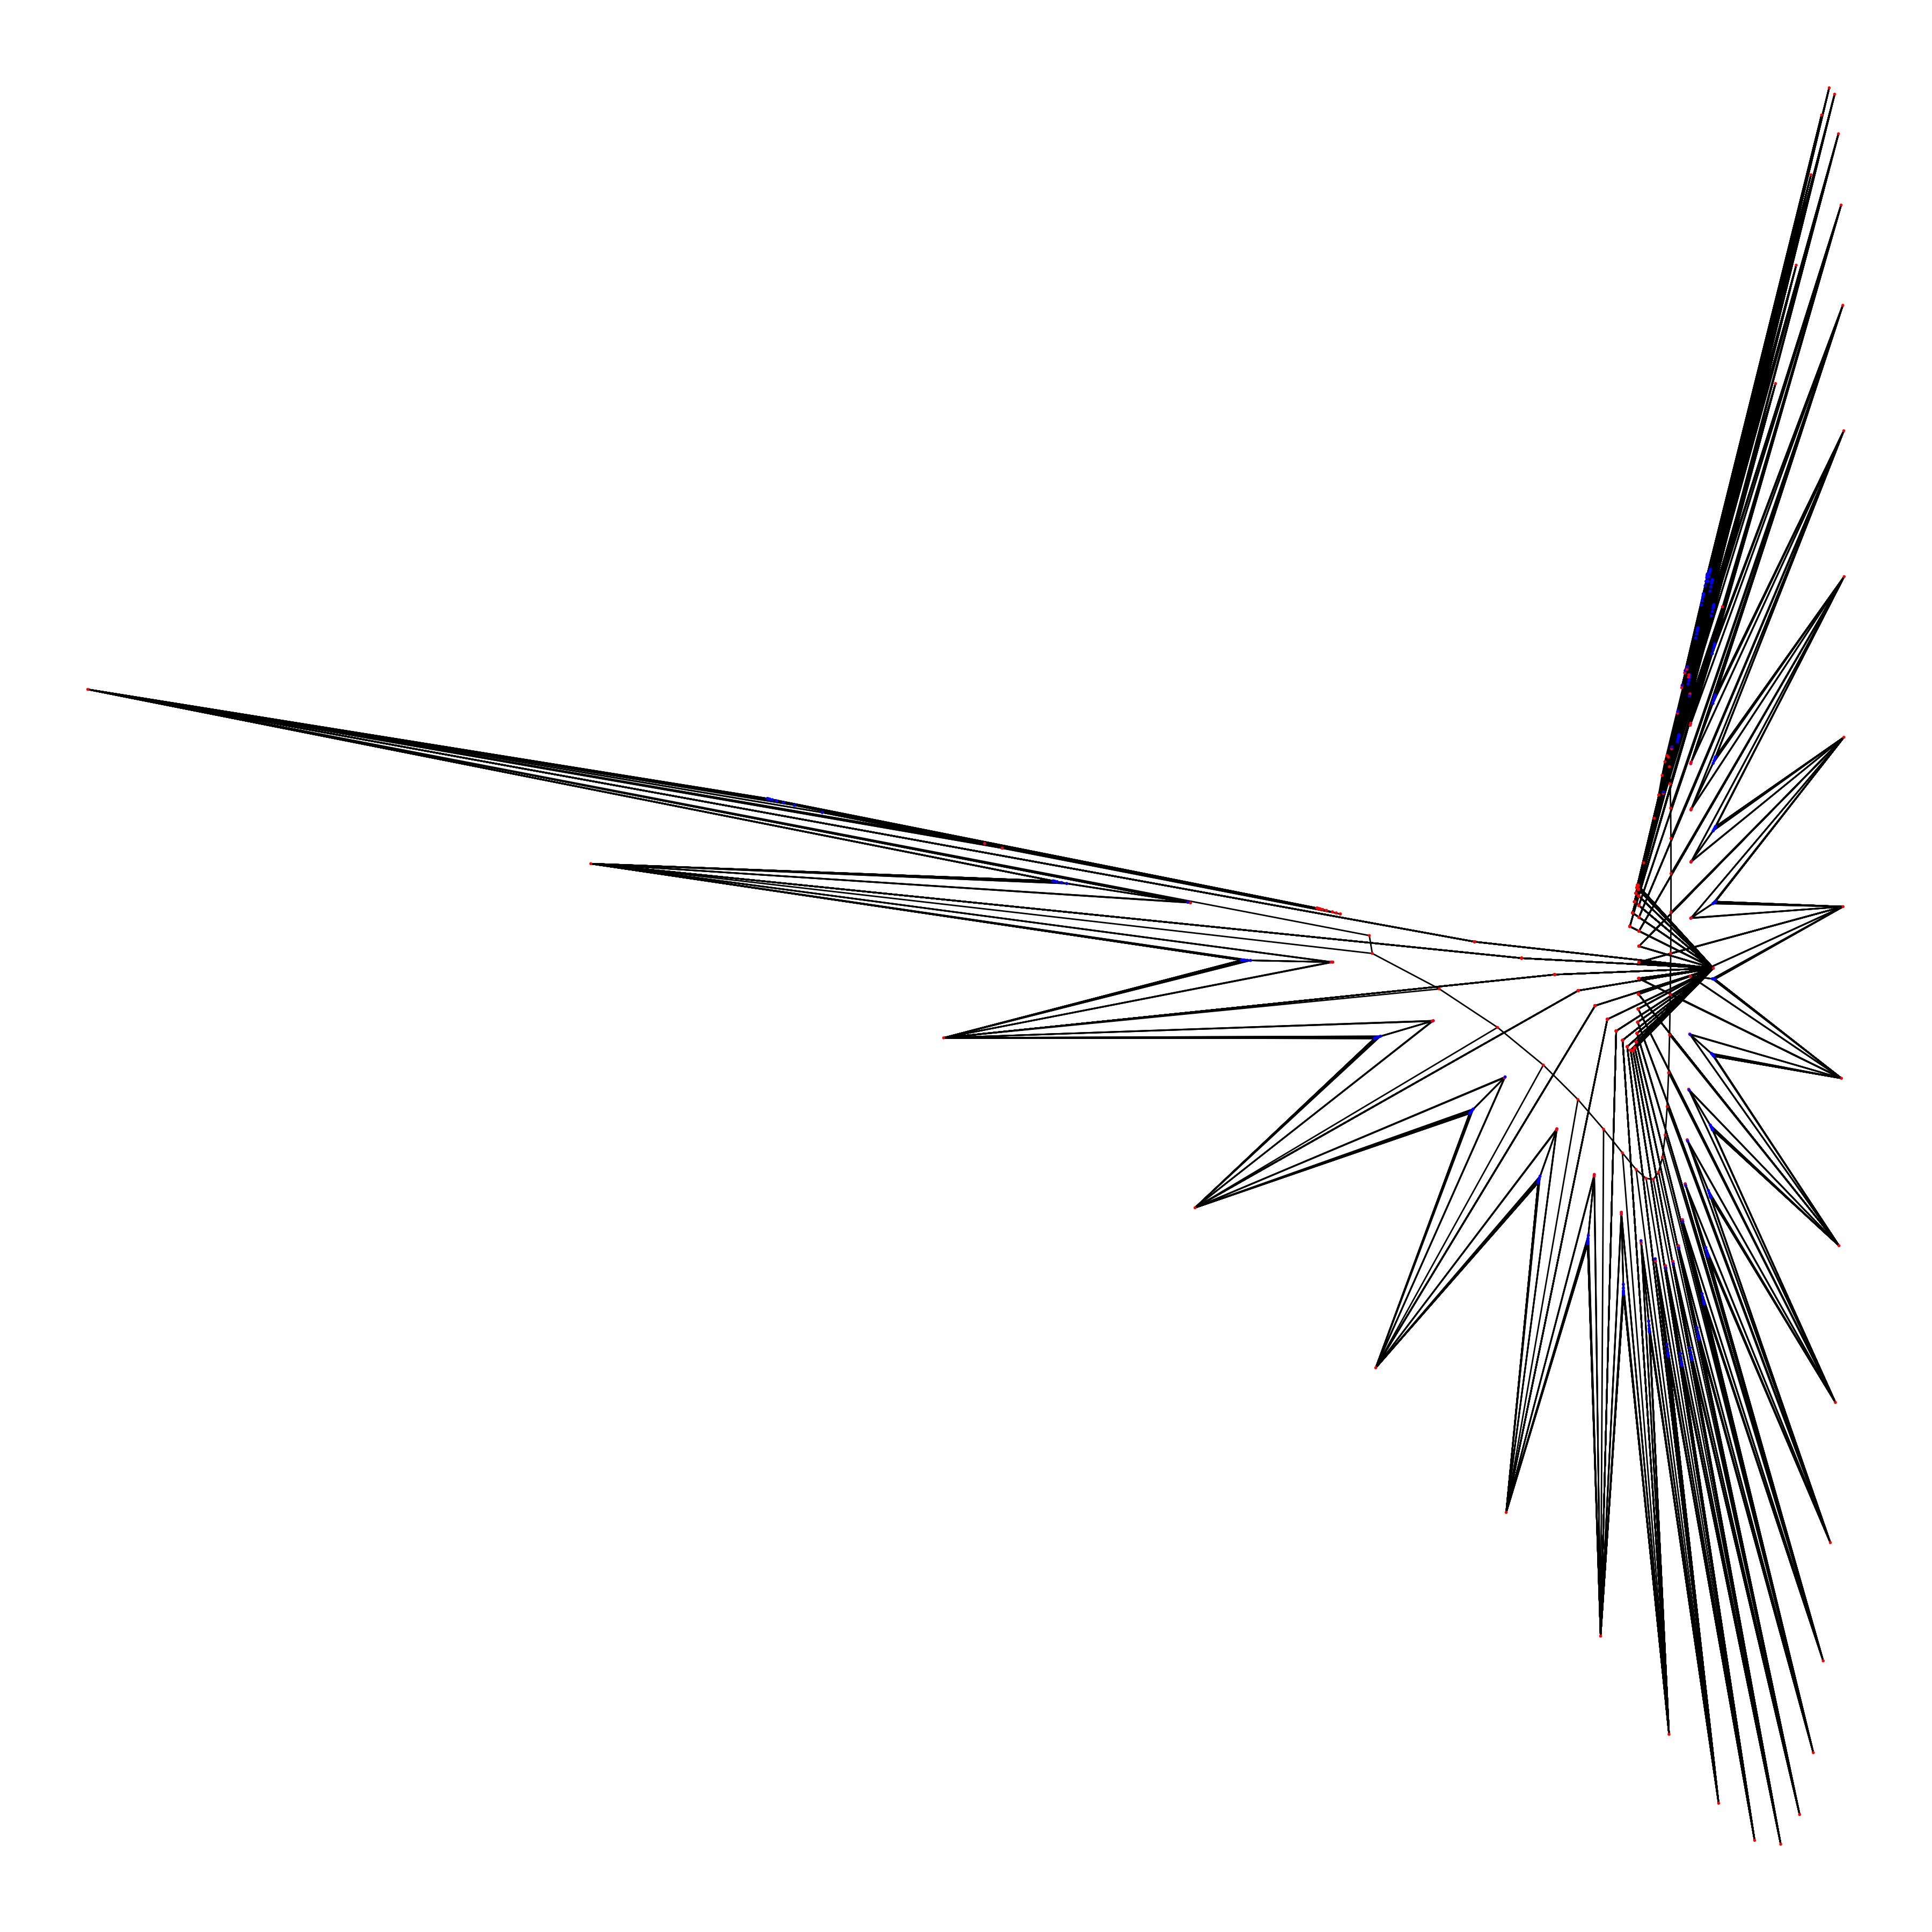
\includegraphics[width=0.75\textwidth]{mygraph_a28o.png}
	\end{figure}
}

\frame{
	\begin{figure}[h]
	\caption{Experiment a28o $|V| = 1365 \quad |E| = 3775$. Uniform weight drawing.}
	\centering
	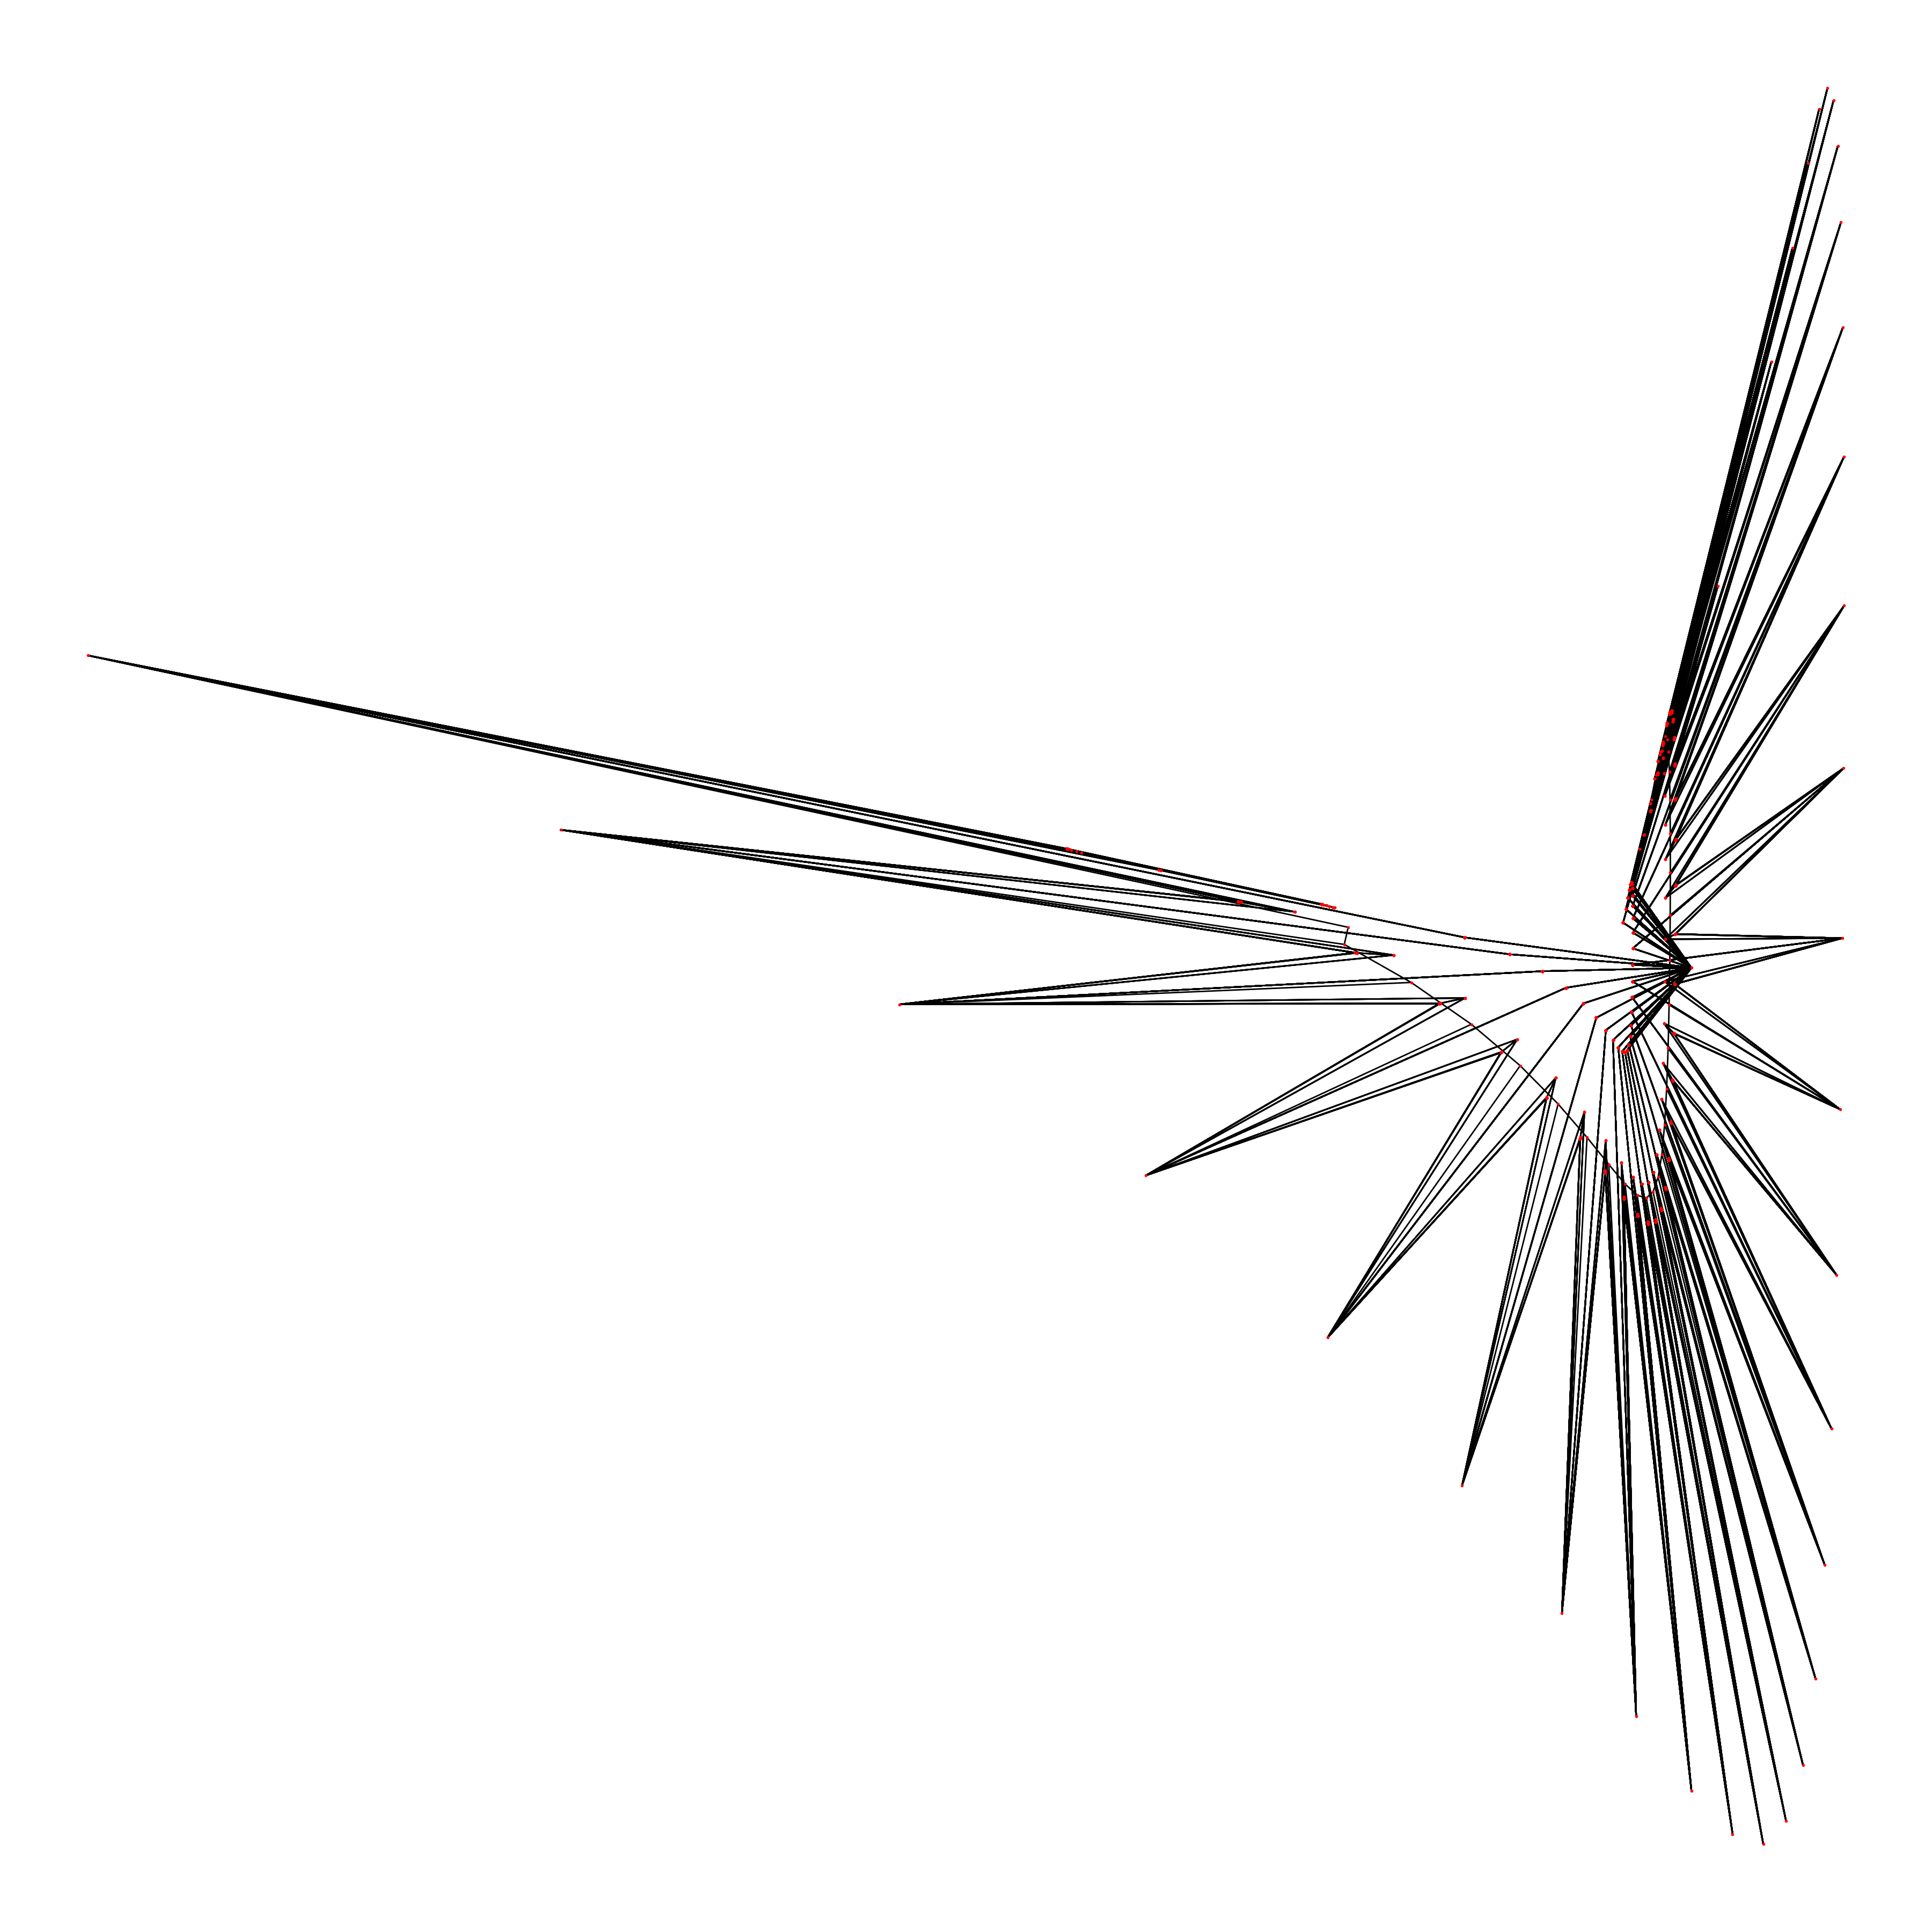
\includegraphics[width=0.75\textwidth]{mygraph_a28o_nw.png}
	\end{figure}
}

\frame{
	\begin{figure}[h]
	\caption{Experiment a2dn $|V| = 2106 \quad |E| = 3603$. Weighted drawing.}
	\centering
	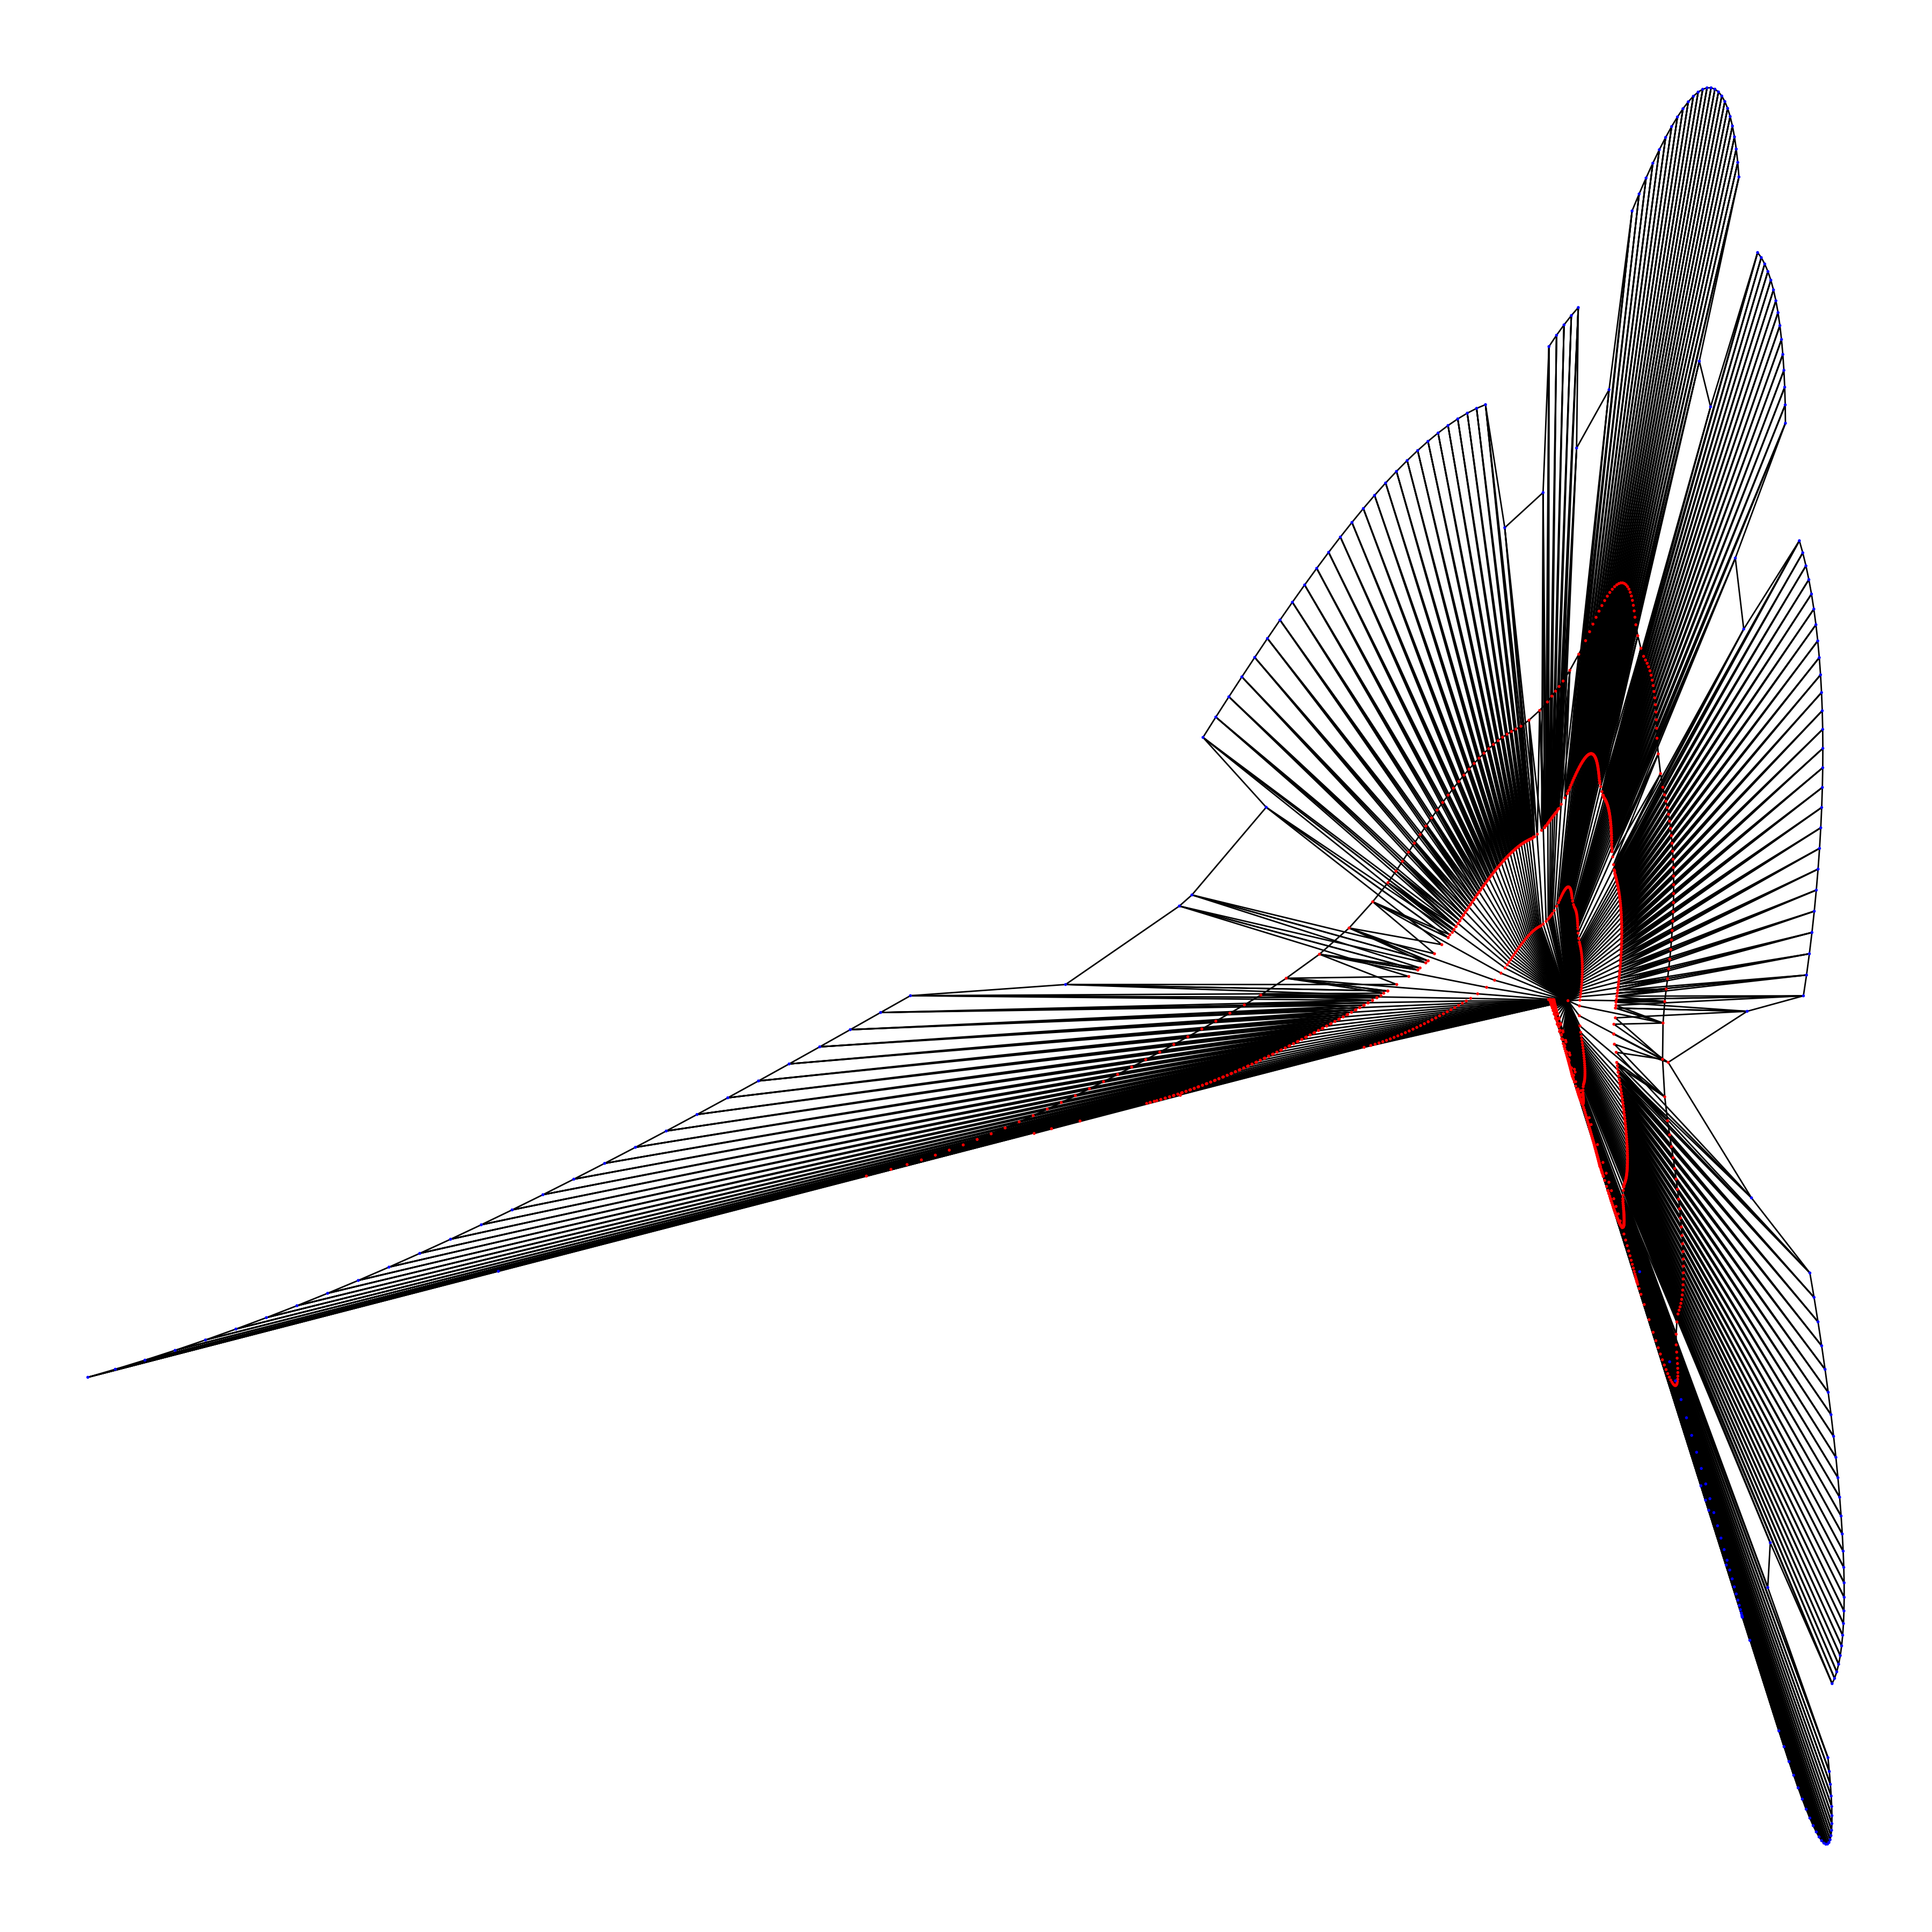
\includegraphics[width=0.75\textwidth]{mygraph_a2dn.png}
	\end{figure}
}

\frame{
	\begin{figure}[h]
	\caption{Experiment a2dn $|V| = 2106 \quad |E| = 3603$. Uniform weight drawing.}
	\centering
	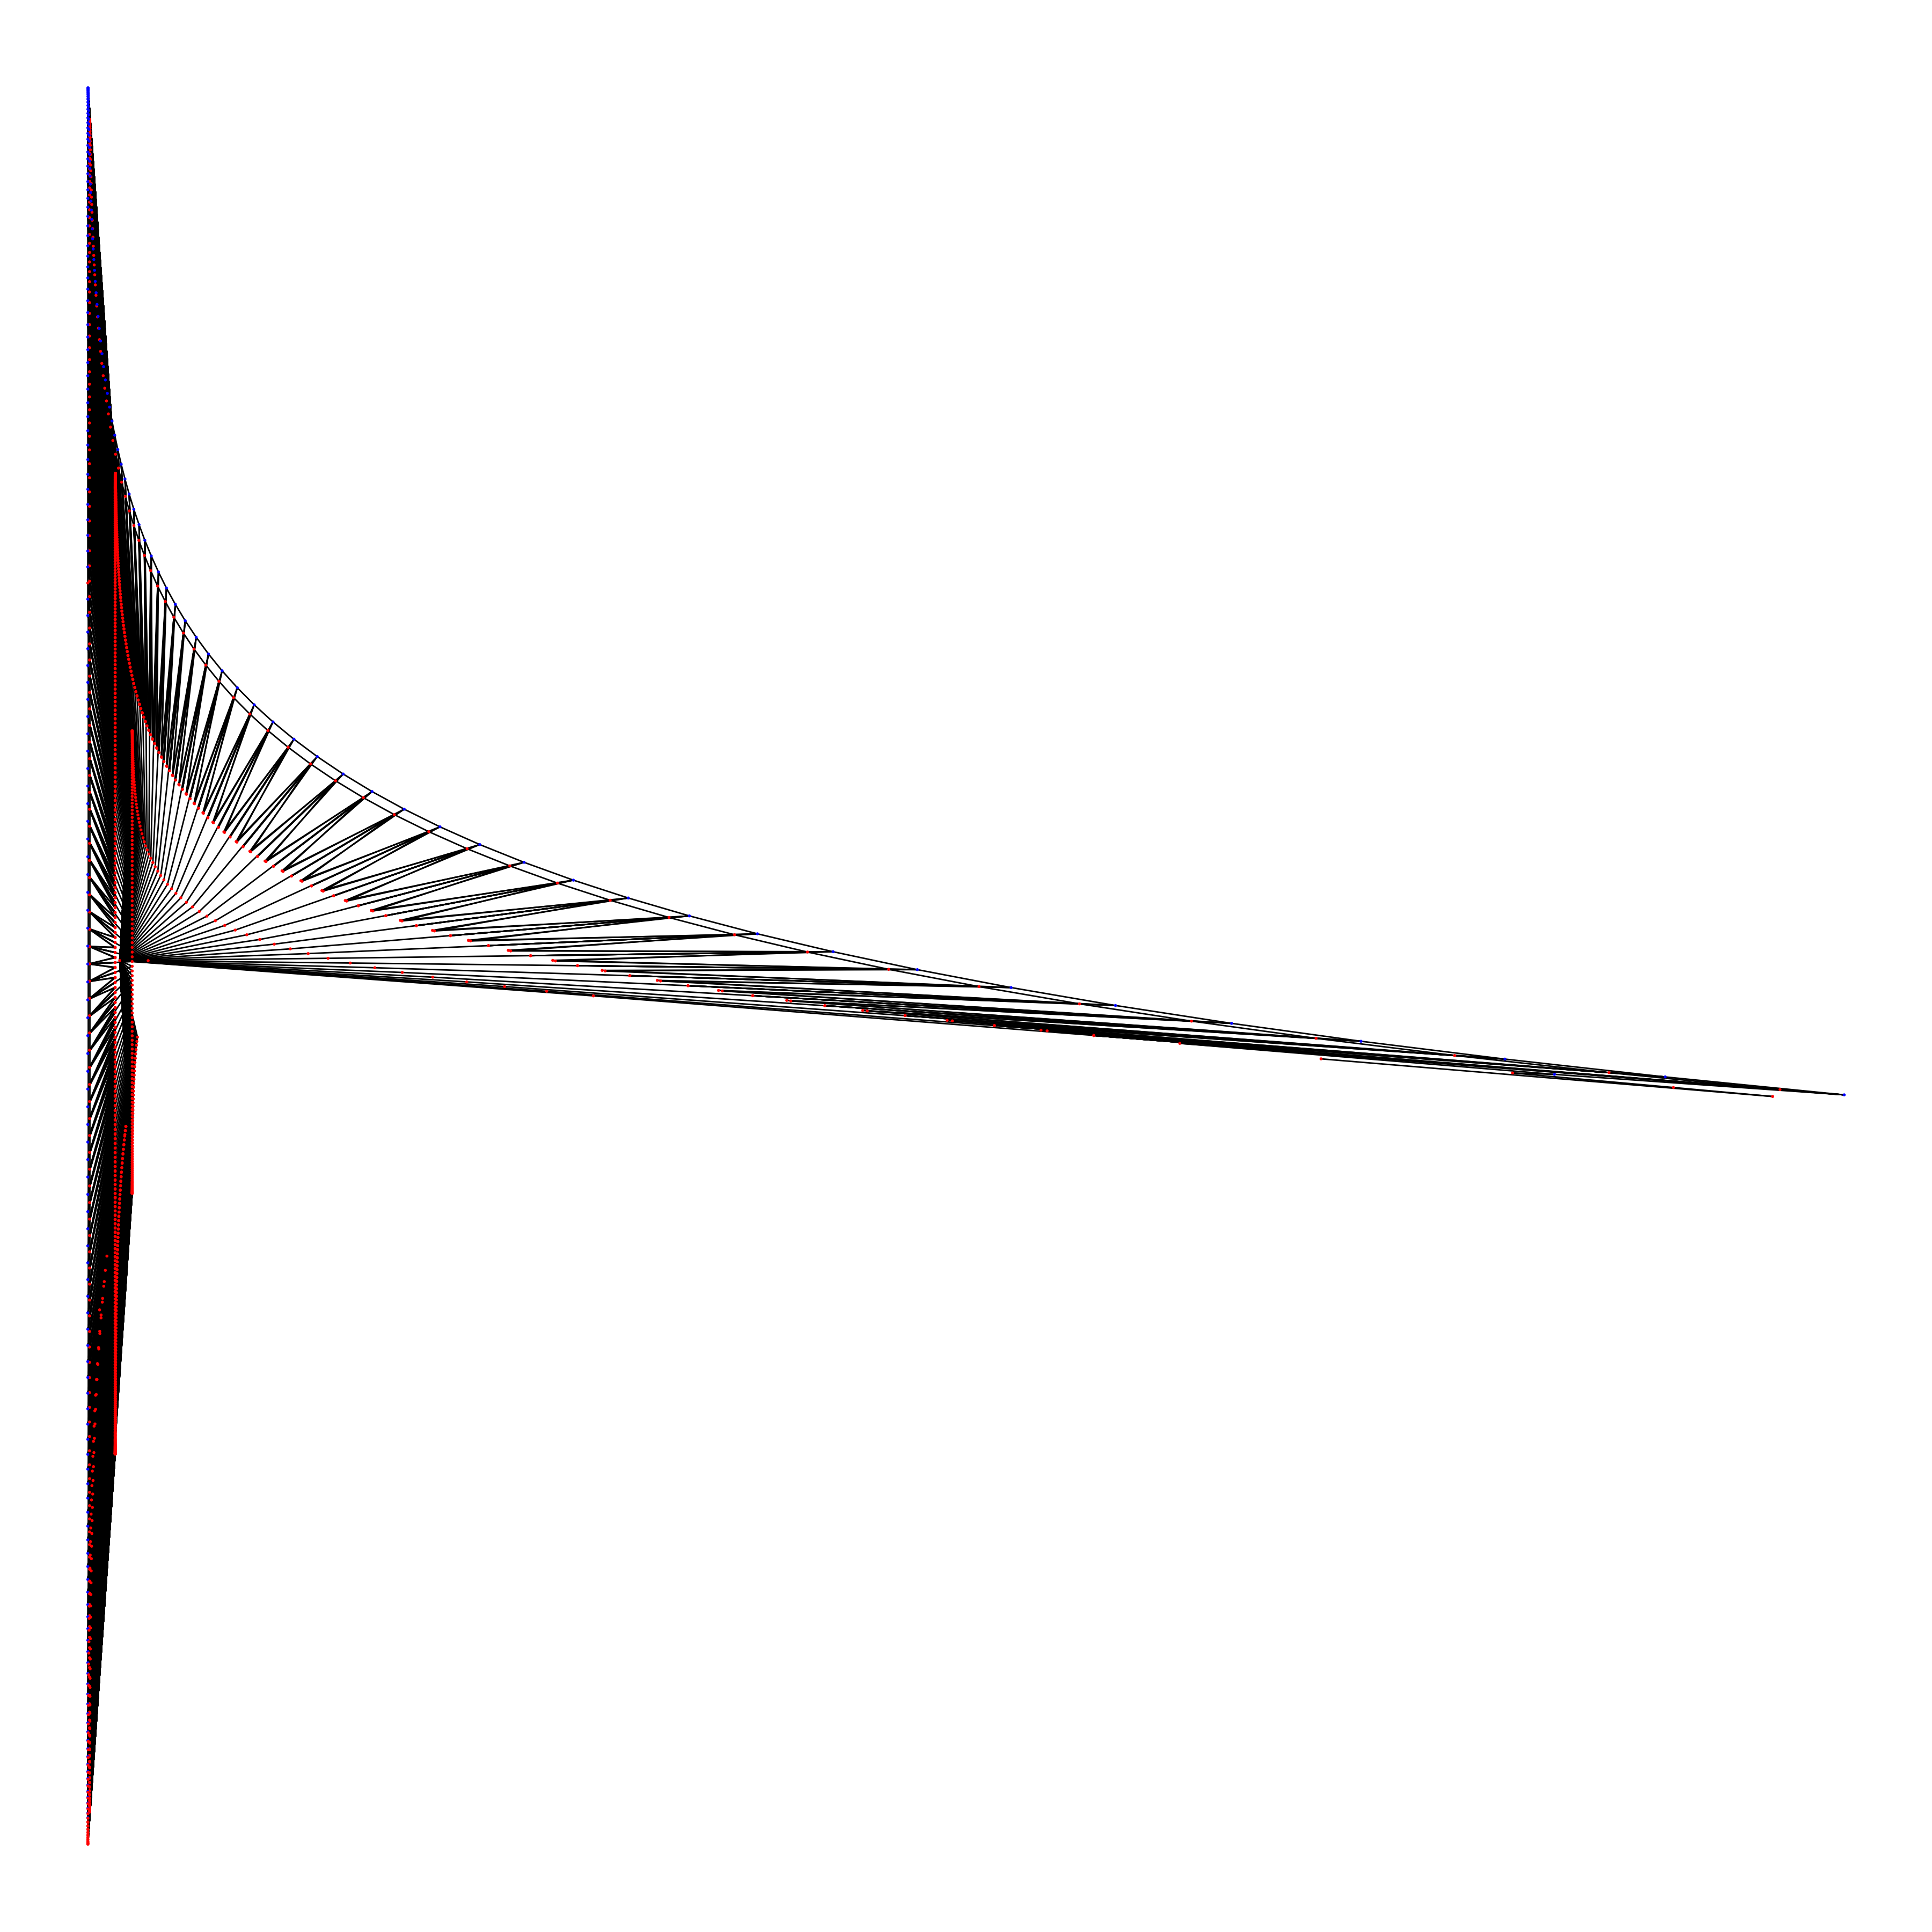
\includegraphics[width=0.75\textwidth]{mygraph_a2dn_nw.png}
	\end{figure}
}

\frame{
	All the previous experiments were completed in under 1 second.
}

\frame{
	\begin{figure}[h]
	\caption{Barabasi-Albert Model $|V| = 30000 \quad |E| = 29999$. Uniform weight drawing. Eigenvectors computed in 16.52s.}
	\centering
	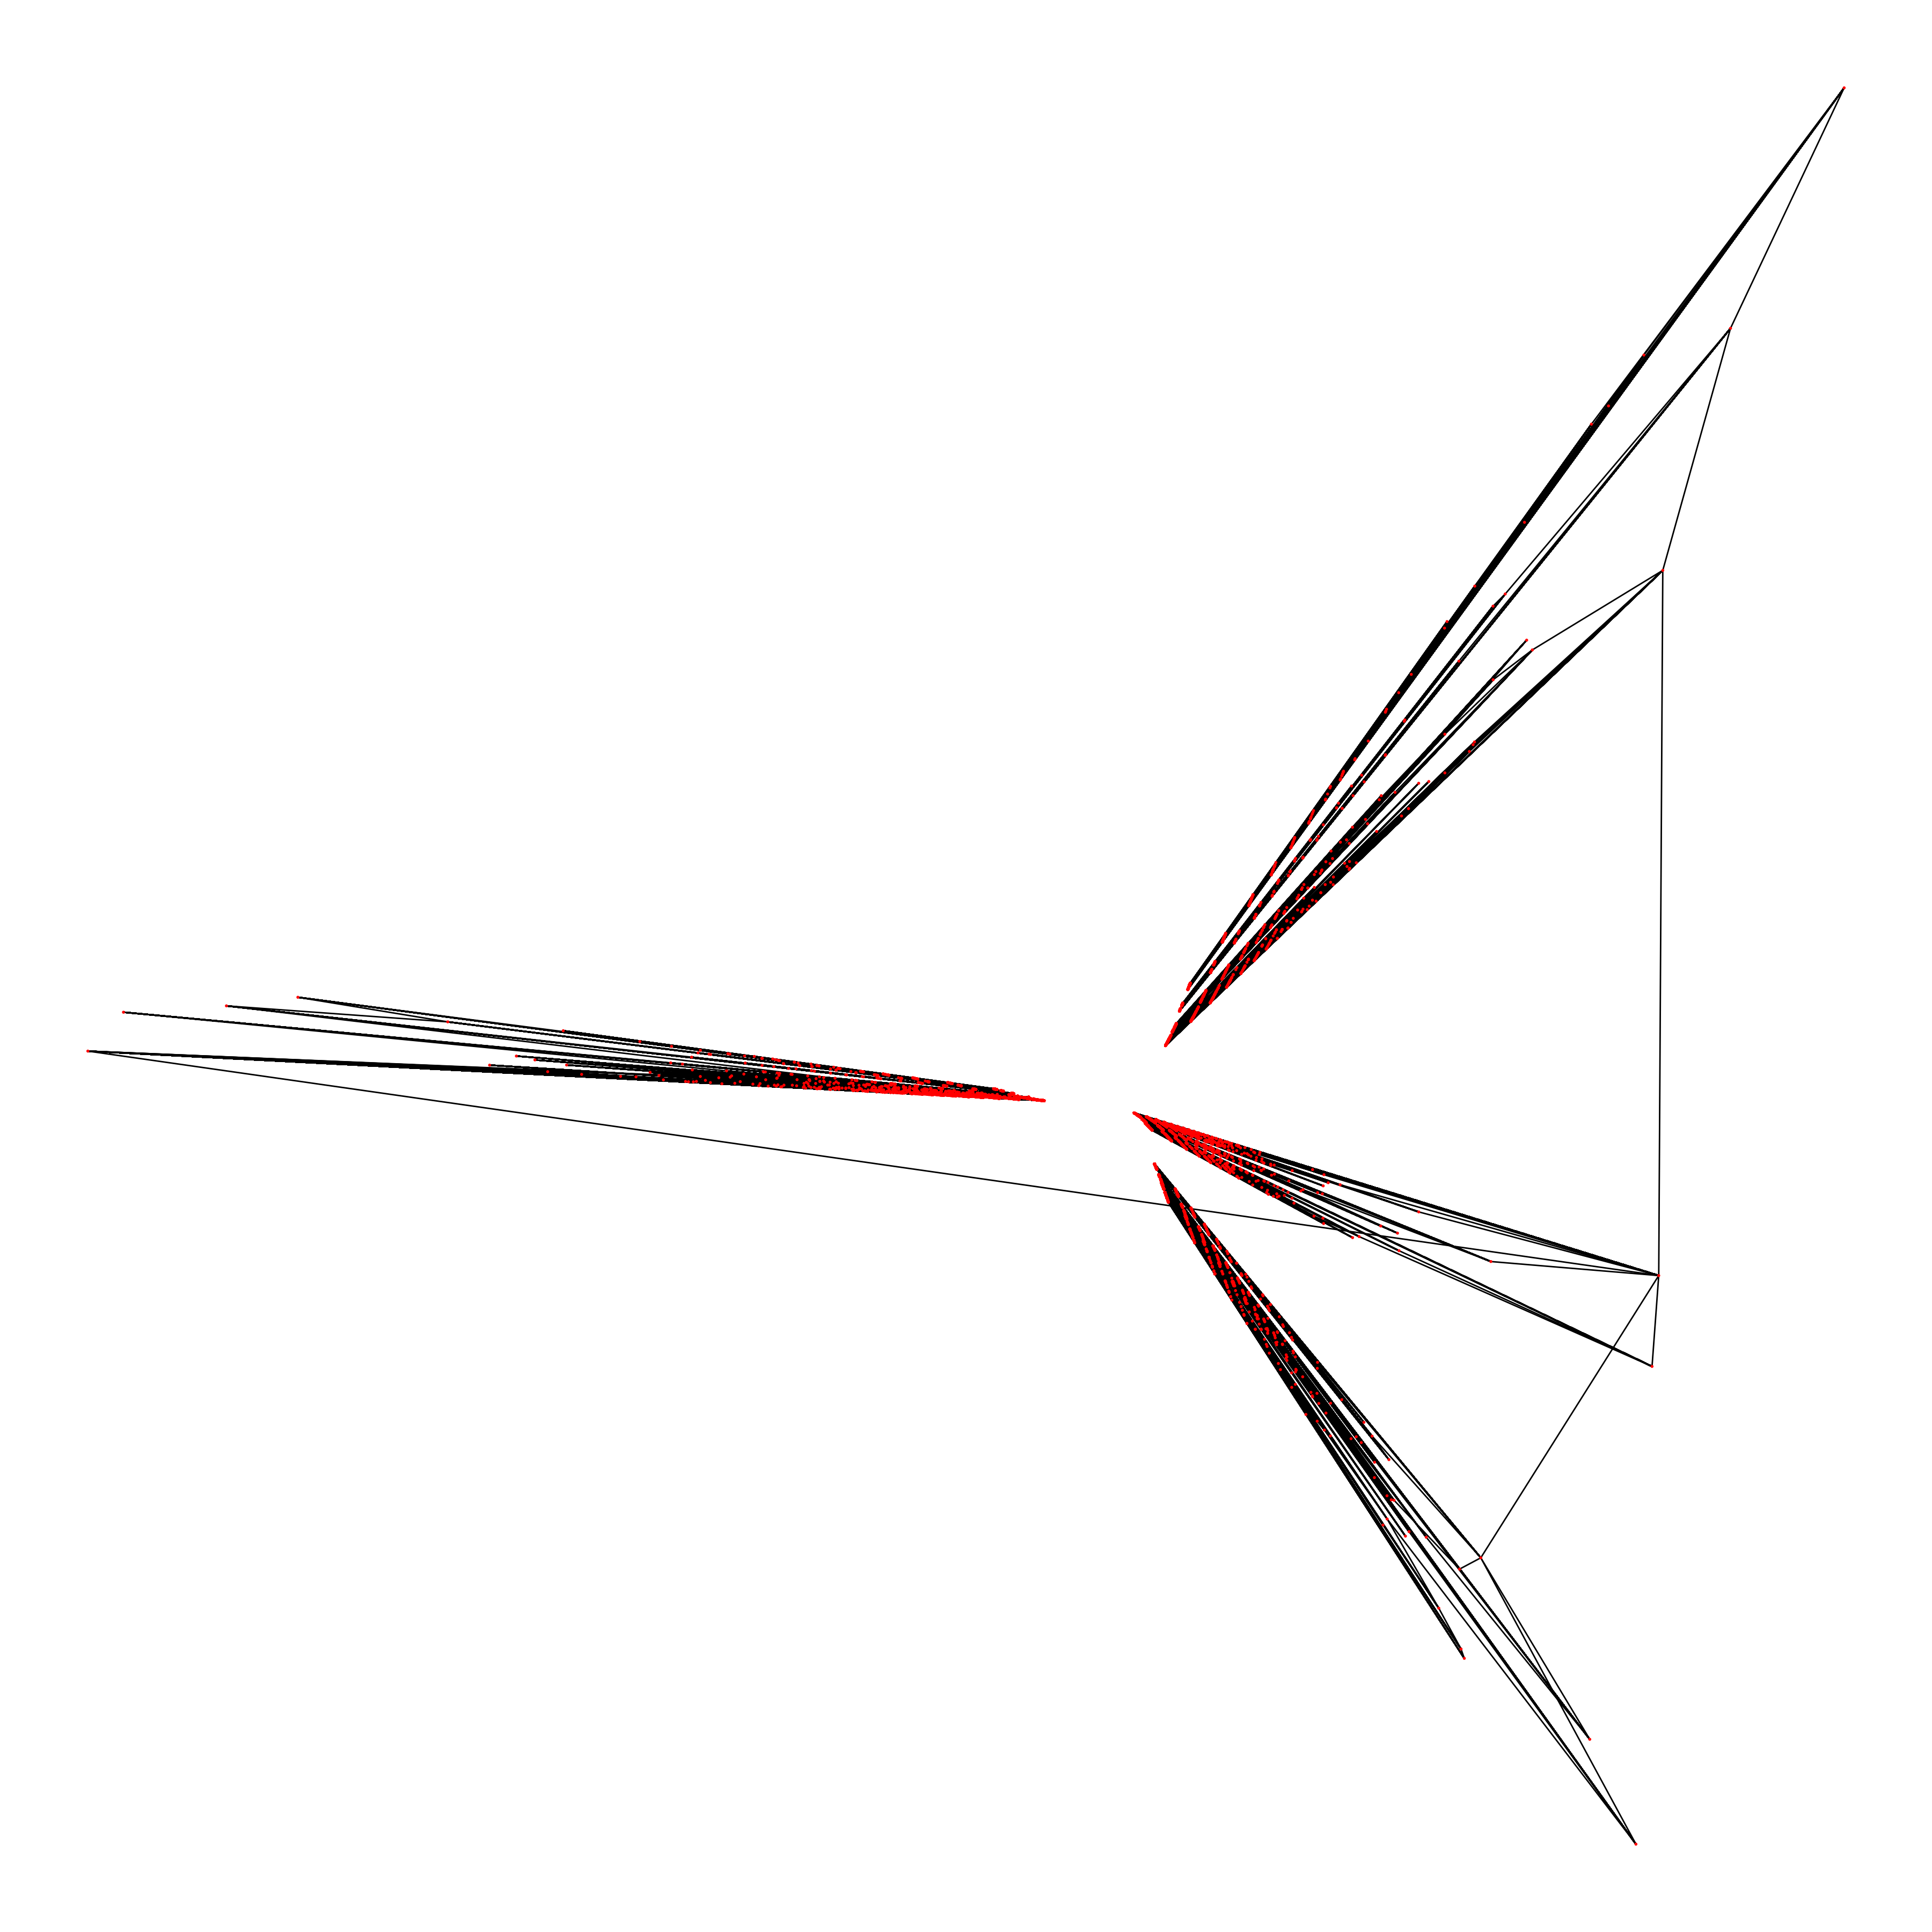
\includegraphics[width=0.75\textwidth]{mygraph_bamodel30k.png}
	\end{figure}
}

\frame{
	\begin{figure}[h]
	\caption{Erdos-Renyi Model ($p = 0.001$) $|V| = 30000 \quad |E| = 448985$. Uniform weight drawing. Eigenvectors computed in 5.94s.}
	\centering
	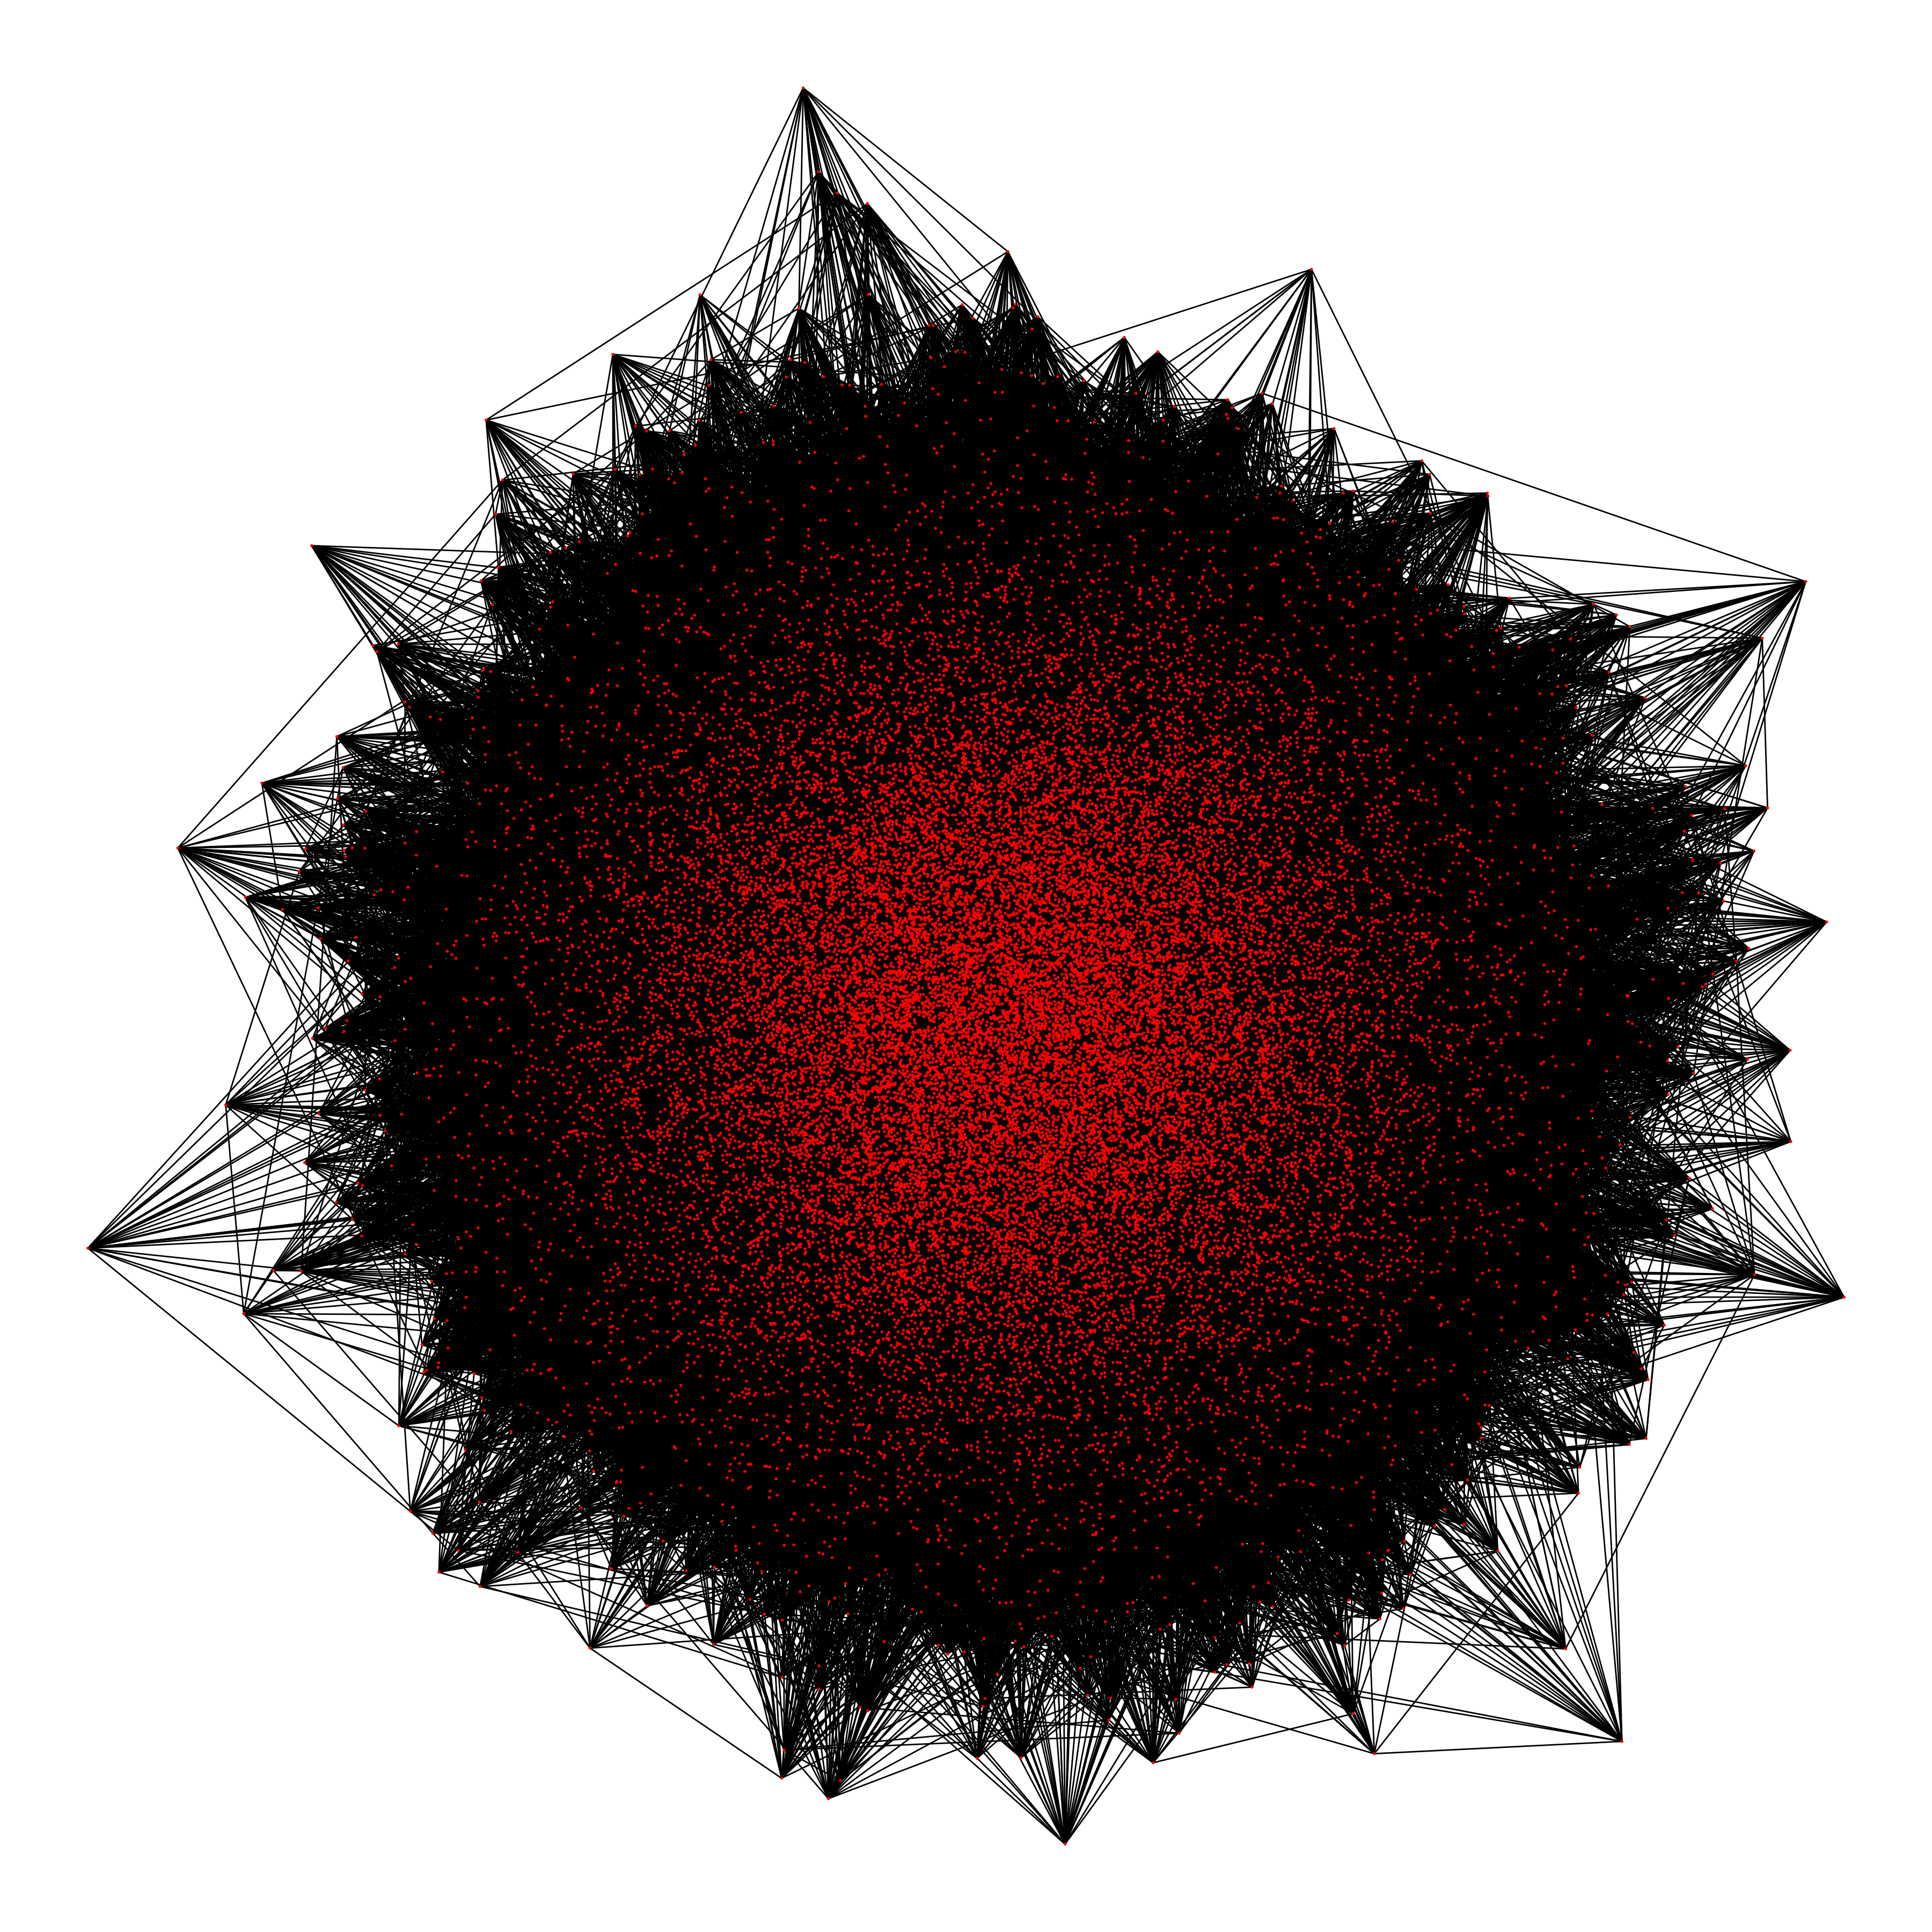
\includegraphics[width=0.75\textwidth]{mygraph_ermodel30k.png}
	\end{figure}
}

\frame{
	Demo Time?
}

\begin{frame}

\begin{thebibliography}{10}
\bibitem{koren}
\alert{Y. Koren}
\newblock  {Drawing Graphs by Eigenvectors: Theory and Practice}
\newblock {\em Computers and Mathematics with Applications 49 (2005) 1867 - 1888}.

\end{thebibliography}
\end{frame}

\end{document}
